\documentclass[border=5mm]{standalone}
\usepackage{amsmath}
\usepackage{tikz}
\usetikzlibrary{arrows.meta, positioning}

\begin{document}
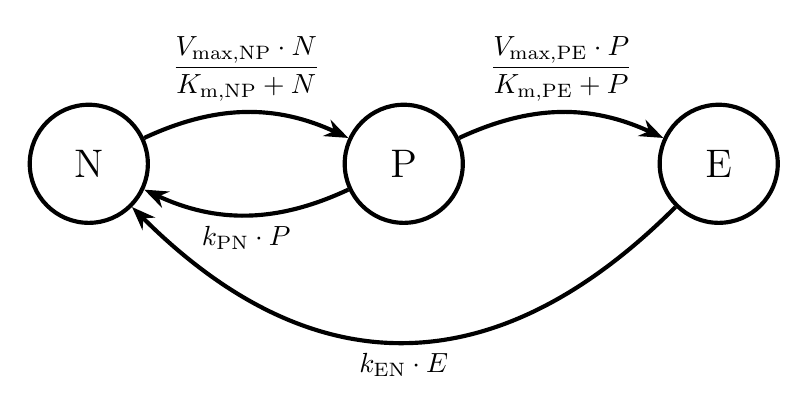
\begin{tikzpicture}[
    node distance=4cm,
    state/.style={circle, draw, minimum size=1.5cm, line width=1.5pt, font=\Large},
    arrow/.style={-{Stealth[length=3mm]}, line width=1.5pt}
]

% Define nodes
\node[state] (N) {N};
\node[state, right of=N] (P) {P};
\node[state, right of=P] (E) {E};

% Define arrows
% N -> P (top curve)
\draw[arrow, bend left=25] (N) to node[midway, above, font=\normalsize] {$\dfrac{V_{\text{max,NP}} \cdot N}{K_{\text{m,NP}}+N}$} (P);

% P -> N (bottom curve)
\draw[arrow, bend left=25] (P) to node[midway, below, font=\normalsize] {$k_{\text{PN}} \cdot P$} (N);

% P -> E (top curve)
\draw[arrow, bend left=25] (P) to node[midway, above, font=\normalsize] {$\dfrac{V_{\text{max,PE}} \cdot P}{K_{\text{m,PE}}+P}$} (E);

% E -> N (large arc underneath)
\draw[arrow] (E) to [out=225, in=315, looseness=1.2] node[midway, below, font=\normalsize] {$k_{\text{EN}} \cdot E$} (N);

\end{tikzpicture}
\end{document}
